%% LaTeX Beamer presentation: Climate and Health Prioritization for TASK
\documentclass{beamer}

% Enhanced packages for better styling
\usepackage{graphicx}
\usepackage{hyperref}
\usepackage{booktabs}
\usepackage{bibentry}
\usepackage{multicol}
\usepackage{xcolor}
\usepackage{fontawesome5}
\usepackage{tikz}
\usepackage{tcolorbox}
\usepackage{listings}
\usepackage{enumitem}
% Define spacing for enumitem to avoid 'spacing undefined' error
\SetEnumitemKey{spacing}{itemsep}

% For including PDF images of diagrams
\usepackage{pdfpages}

% Custom colors
\definecolor{taskblue}{RGB}{0, 83, 155}
\definecolor{tasklightblue}{RGB}{135, 206, 250}
\definecolor{taskgreen}{RGB}{34, 139, 34}
\definecolor{taskred}{RGB}{178, 34, 34}
\definecolor{taskorange}{RGB}{255, 140, 0}

% Theme customization
\usetheme{CambridgeUS}
\usecolortheme{whale}
\setbeamercolor{title}{fg=white, bg=taskblue}
\setbeamercolor{frametitle}{fg=white, bg=taskblue}
\setbeamercolor{structure}{fg=taskblue}
\setbeamercolor{block title}{fg=white, bg=taskblue}
\setbeamercolor{block body}{fg=black, bg=tasklightblue!30}
\setbeamercolor{itemize item}{fg=taskblue}
\setbeamercolor{itemize subitem}{fg=taskorange}

% Title page customization
\title[Climate \& Health for TASK]{\textbf{Decarbonizing Clinical Research:} \\Why Climate and Health Should Be a Strategic Priority for TASK}
\author{\textbf{Craig Parker} \\ \small{Wits Planetary Health, University of the Witwatersrand}}
\date{\textbf{TASK Clinical Trials Afternoon Lecture, 2025}}
% Logo commented out until image available
% \logo{\includegraphics[height=1cm]{example-image}}

% Custom commands for consistent styling
\newcommand{\highlight}[1]{\textcolor{taskred}{\textbf{#1}}}
\newcommand{\source}[1]{\vspace{0.3cm}\hfill\scriptsize\textcolor{gray}{Source: #1}}

% Custom block environments
\newenvironment{impactblock}{\begin{tcolorbox}[colback=taskorange!20, colframe=taskorange, title=\textbf{Key Impact}]}{\end{tcolorbox}}
\newenvironment{actionblock}{\begin{tcolorbox}[colback=taskgreen!20, colframe=taskgreen, title=\textbf{Action Item}]}{\end{tcolorbox}}

\begin{document}

% Title page with simple styling
\begin{frame}[plain]
\titlepage

% Instead of using TikZ for the footer, we'll use a simple colored box
\vspace*{\fill}
\begin{beamercolorbox}[wd=\paperwidth,ht=1cm,dp=0ex]{structure.fg}
  \hfill{\small\textcolor{white}{Climate \& Health Initiative}}\hspace{0.5cm}\strut
\end{beamercolorbox}
\end{frame}

% Slide 1: Using Climate Health Impact Flow Diagram
\begin{frame}{Why Climate and Health Matter}
    % Replace icons with comprehensive flow diagram
    % Check if image exists before including
\IfFileExists{diagrams/pdf/climate_health_impact_flow.png}{%
    \includegraphics[width=\textwidth,height=0.7\textheight]{diagrams/pdf/climate_health_impact_flow.png}%
}{%
    \centering\Large\textbf{[Climate Health Impact Flow Diagram]}%
    \vspace{2cm}%
}
    
    \begin{impactblock}
    Climate change threatens to reverse decades of progress in global health outcomes
    \end{impactblock}
    
    \source{The Lancet Countdown, 2023}
\end{frame}

% Slide 2: Using South Africa's Climate Vulnerability Map
\begin{frame}{South Africa's Exposure}
    % Replace pie chart with vulnerability map
    % Check if image exists before including
\IfFileExists{diagrams/pdf/sa_climate_vulnerability_map.png}{%
    \includegraphics[width=\textwidth,height=0.8\textheight]{diagrams/pdf/sa_climate_vulnerability_map.png}%
}{%
    \centering\Large\textbf{[South Africa Climate Vulnerability Map]}%
    \vspace{2cm}%
}
    
    \source{Lancet Countdown South Africa Country Profile, 2023}
\end{frame}

% Slide 3: Using Research Emissions Sankey Diagram
\begin{frame}{Research Sector's Role in Emissions}
    % Replace table and image with Sankey diagram
    % Check if image exists before including
\IfFileExists{diagrams/pdf/research_emissions_sankey.png}{%
    \includegraphics[width=\textwidth,height=0.8\textheight]{diagrams/pdf/research_emissions_sankey.png}%
}{%
    \centering\Large\textbf{[Research Emissions Sankey Diagram]}%
    \vspace{2cm}%
}
    
    \source{Nature, 2021: d41586-021-02696-6}
\end{frame}

% Slide 4: Using Funding Priorities Venn Diagram
\begin{frame}{Why Funders Care}
    \begin{tcolorbox}[colback=white, colframe=taskblue, title=\textbf{Wellcome Trust Policy}]
    \centering
    \textit{"Only fund research conducted in an environmentally sustainable way."}
    \end{tcolorbox}
    
    % Replace text with Venn diagram
    % Check if image exists before including
\IfFileExists{diagrams/pdf/funding_priorities_venn.png}{%
    \includegraphics[width=\textwidth,height=0.65\textheight]{diagrams/pdf/funding_priorities_venn.png}%
}{%
    \centering\Large\textbf{[Funding Priorities Venn Diagram]}%
    \vspace{2cm}%
}
    
    \source{Wellcome Trust Environmental Sustainability Policy}
\end{frame}

% Slide 5: Strategic Benefits with visual enhancement
\begin{frame}{Strategic Benefits for TASK}
\begin{columns}
\column{0.7\textwidth}
\begin{itemize}[itemsep=1em]
    \item \faIcon{chart-line} Strengthens relevance \& resilience of research
    \item \faIcon{handshake} Aligns with global and national climate-health agendas
    \item \faIcon{award} Improves funder competitiveness
    \item \faIcon{dollar-sign} Enhances operational efficiency
\end{itemize}
\column{0.3\textwidth}
\includegraphics[width=\textwidth]{example-image-b} % Replace with WHO logo or relevant image
\end{columns}

% Simplified logo placement
\begin{flushright}
\includegraphics[width=2cm]{example-image} % Replace with relevant logo
\end{flushright}

\source{WHO COP26 Health Programme}
\end{frame}

% Slide 6: Using Green Trial Design Framework
\begin{frame}{What Can TASK Do?}
    % Replace boxes with framework diagram
    % Check if image exists before including
\IfFileExists{diagrams/pdf/green_trial_design_framework.png}{%
    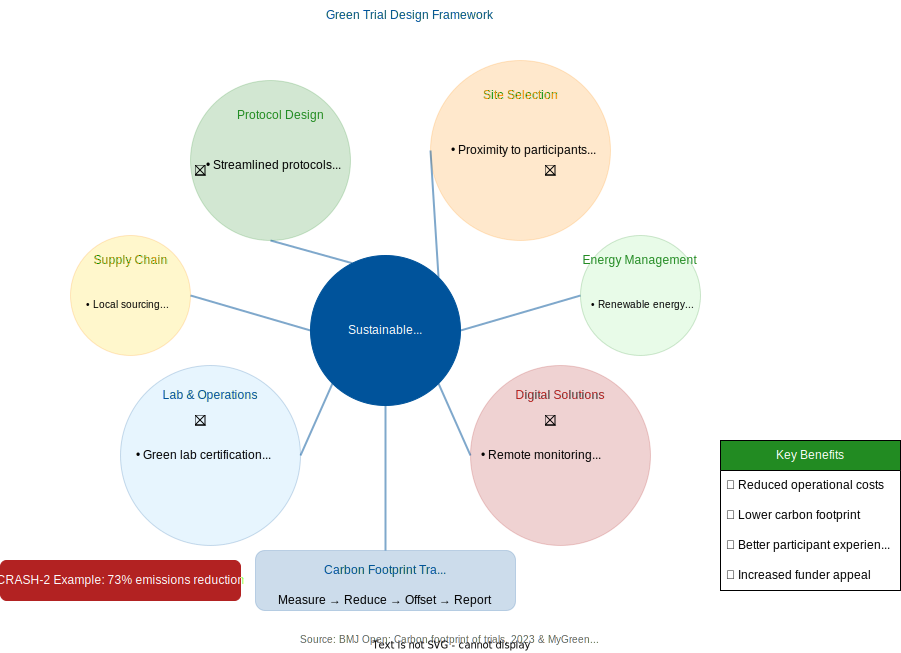
\includegraphics[width=\textwidth,height=0.8\textheight]{diagrams/pdf/green_trial_design_framework.png}%
}{%
    \centering\Large\textbf{[Green Trial Design Framework]}%
    \vspace{2cm}%
}
    
    \source{MyGreenLab.org}
\end{frame}

% Slide 7: Using ULT Freezer Temperature-Energy Curve
\begin{frame}{Lab Sustainability in Action}
    % Replace temperature graphic with detailed curve
    % Check if image exists before including
\IfFileExists{diagrams/pdf/freezer_temperature_energy_curve.png}{%
    \includegraphics[width=\textwidth,height=0.8\textheight]{diagrams/pdf/freezer_temperature_energy_curve.png}%
}{%
    \centering\Large\textbf{[Freezer Temperature Energy Curve]}%
    \vspace{2cm}%
}
    
    \begin{actionblock}
    Simple changes in lab practices can reduce energy use by up to 40\%
    \end{actionblock}
    
    \source{Royal Society of Chemistry: Sustainable Laboratories Report}
\end{frame}

% Slide 8: Using CRASH Trials Comparative Dashboard
\begin{frame}{Practical Examples}
    % Replace table with dashboard
    % Check if image exists before including
\IfFileExists{diagrams/pdf/crash_trials_dashboard.png}{%
    \includegraphics[width=\textwidth,height=0.8\textheight]{diagrams/pdf/crash_trials_dashboard.png}%
}{%
    \centering\Large\textbf{[CRASH Trials Dashboard]}%
    \vspace{2cm}%
}
    
    \source{BMJ Open: Carbon footprint of trials, 2023}
\end{frame}

% Slide 9: Using Climate-Health Action Roadmap
\begin{frame}{Conclusion}
    \begin{center}
    \Large\textbf{\textcolor{taskblue}{Healing without harming}}
    \end{center}
    
    % Replace icon and next steps box with roadmap
    % Check if image exists before including
\IfFileExists{diagrams/pdf/climate_health_roadmap.png}{%
    \includegraphics[width=\textwidth,height=0.7\textheight]{diagrams/pdf/climate_health_roadmap.png}%
}{%
    \centering\Large\textbf{[Climate Health Action Roadmap]}%
    \vspace{2cm}%
}
    
    \begin{itemize}[itemsep=0.7em]
        \item Climate-health is \highlight{core} to effective research
        \item TASK can lead on low-carbon trials in Africa
    \end{itemize}
\end{frame}

% Slide 10: References with better formatting
\begin{frame}[allowframebreaks]{References}
\begin{thebibliography}{99}
\bibitem{lancet}
\textbf{The Lancet Countdown} (2023).
\textit{The 2023 report of the Lancet Countdown on health and climate change.}
\url{https://www.thelancet.com/countdown-health-climate}

\bibitem{lancetsa}
\textbf{Lancet Countdown} (2023).
\textit{South Africa Country Profile.}
\url{https://www.lancetcountdown.org/south-africa-country-profile}

\bibitem{nature}
\textbf{Wallis, S. et al.} (2021).
\textit{Clinical trials: Rethinking how we reduce carbon emissions.}
Nature, 597(7878), 637.

\bibitem{wellcome}
\textbf{Wellcome Trust} (2023).
\textit{Environmental Sustainability Policy.}
\url{https://wellcome.org/grant-funding/guidance/environmental-sustainability-policy}

\bibitem{who}
\textbf{World Health Organization} (2021).
\textit{COP26 Health Programme.}
\url{https://www.who.int/initiatives/cop26-health-programme}

\bibitem{greenlab}
\textbf{My Green Lab} (2023).
\textit{Laboratory Sustainability Best Practices.}
\url{https://www.mygreenlab.org}

\bibitem{rsc}
\textbf{Royal Society of Chemistry} (2022).
\textit{Sustainable Laboratories Report.}
\url{https://www.rsc.org/sustainable-laboratories-report}

\bibitem{bmj}
\textbf{Roberts I. et al.} (2023).
\textit{Carbon footprint of randomised controlled trials: retrospective study of CRASH trials.}
BMJ Open, 13(5):e070648.
\end{thebibliography}
\end{frame}

% Final slide
\begin{frame}[plain]
\begin{center}
\vspace{1cm}
{\Large\textbf{Thank you}}

\vspace{0.5cm}
{\large Questions?}

\vspace{1cm}
\faEnvelope\ craig.parker@wits.ac.za\\
\faTwitter\ @WitsPlanetaryHealth
\end{center}

% Simplified logo placement
\begin{center}
\vspace{1cm}
% \includegraphics[width=6cm]{example-image} % Commented out until logos available
\textbf{[Institution logos]}
\end{center}
\end{frame}

\end{document}